\documentclass[a4paper,graphics,11pt]{article}
\pagenumbering{arabic}

\usepackage[margin=1in]{geometry}
\usepackage[utf8]{inputenc}
\usepackage[T1]{fontenc}
\usepackage{lmodern}
\usepackage[ngerman]{babel}
\usepackage{amsmath, tabu}
\usepackage{amsthm}
\usepackage{amssymb}
\usepackage{complexity}
\usepackage{mathtools}
\usepackage{setspace}
\usepackage{graphicx,color,curves,epsf,float,rotating}
\usepackage{tasks}

\setlength{\parindent}{0em}
\setlength{\parskip}{1em}

\newcommand\aufgabe[1]{\subsection*{Aufgabe #1}}

\begin{document}
\noindent Gruppe \fbox{\textbf{11}}             \hfill Tobias Riedel, 379133 \\
\noindent Analysis für Informatiker             \hfill Phil Pützstück, 377247 \\

\begin{center}
	\LARGE{\textbf{Hausaufgabe 2}}
\end{center}
\begin{center}
\rule[0.1ex]{\textwidth}{1pt}
\end{center}



\aufgabe{1}
\begin{tasks}(1)
    \task \\ 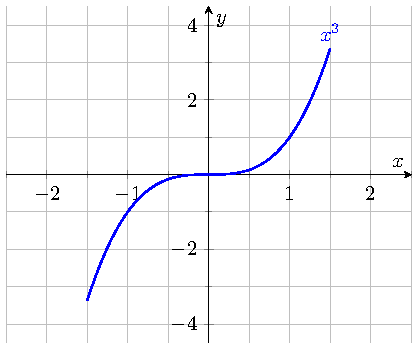
\includegraphics{graphics/graph0.pdf}
        \\ \\ 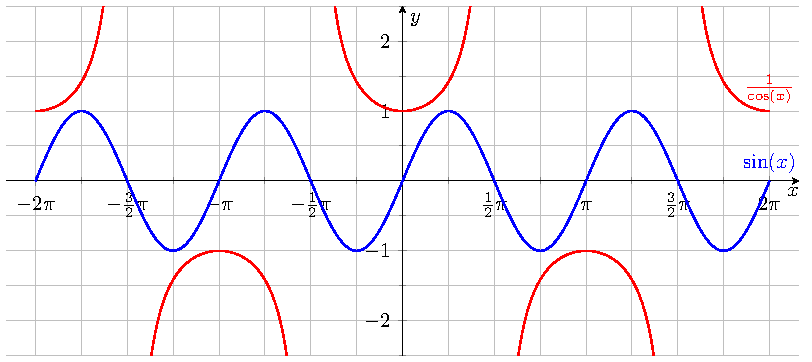
\includegraphics{graphics/graph1.pdf}\\\\
        \textbf{Hinweis} zur Notation und Wortwahl.
        Es werden folgende Definitionen angenommen:
        \begin{itemize}
            \item Abbildung $f \colon $ Definitionsbereich $\mapsto$ Zielbereich.
            \item Wertebereich bzw. Wertemenge ist die Menge angenommener Werte der Funktion.
            \item (Wertebereich $\subseteq$ Zielbereich)
                ist stets erfüllt.
            \item Bsp. $\sin(x)$: Zielbereich ist $\mathbb{R}$, Wertebereich ist $[-1,1]$
        \end{itemize}


    \task   \begin{itemize}
        \item $f \colon \mathbb{R} \rightarrow \mathbb{R},\ x \mapsto x^3$,
            Wertebereich $\mathbb{R}$
        \item $g \colon \mathbb{R} \rightarrow \mathbb{R},\ x \mapsto \sin(x)$,
            Wertebereich $[-1,1]$ 
        \item $h \colon \mathbb{R} \setminus \{x \in \mathbb{R} \vert \cos(x) = 0\} \rightarrow \mathbb{R} ,\ x \mapsto \frac{1}{\cos(x)}$, Wertebereich $\mathbb{R} \setminus (-1,1)$
            \end{itemize}

    \task\\
        $f \colon \mathbb{R} \rightarrow \mathbb{R}$
        ist bijektiv, d.h. $f$ ist injektiv und surjektiv, da jede
        parallele zur x-Achse genau einen Schnittpunkt mit dem Graphen
        von $f$ hat. Jeder Wert im Zielbereich $\mathbb{R}$ wird mindesten
        und höchstens einmal getroffen. Somit ist der Wertebereich gleich dem
        Zielbereich.\\

        $g \colon \mathbb{R} \rightarrow \mathbb{R}$
        ist weder injektiv noch surjektiv. Es werden nur Werte im
        Wertebereich $[-1,1]$ getroffen, welcher hier eine echte Teilmenge des
        Zielbereiches $\mathbb{R}$ ist.
        Weiterhin werden die Werte des Wertebereichs unendlich oft getroffen:
        $$\forall x \in \mathbb{R},\,\forall n \in \mathbb{Z}\colon\sin(x) = \sin(x+2n\pi)\ $$
        Dies ist auch an der wiederholenden Wellenform des Graphen zu erkennen.\\

    \task\\Bijektive Abbildungen, Wertebereich ist notwendigerweise gleich dem Zielbereich:
        \begin{itemize}
            \item $f: \mathbb{R} \rightarrow \mathbb{R}, x \mapsto x^3$
            \item $g: [-\frac{\pi}{2}, \frac{\pi}{2}] \rightarrow [-1,1], x \mapsto \sin(x)$
            \item $h: [0,\pi] \rightarrow \mathbb{R} \setminus (-1,1), x \mapsto \frac{1}{\cos(x)}$
        \end{itemize}
\end{tasks}


\aufgabe{2}
\begin{tasks}
    \task\\
        $i \colon \mathbb{Z} \rightarrow \mathbb{N}_{0},\ i(x) := \vert x\vert$\\
        ist surjektiv, da $i(-x) = \vert-x\vert = x = \vert x\vert = i(x)$ gilt,
        und somit jeder Wert (außer 0) im Zielbereich $\mathbb{N}_{0}$ zwei mal getroffen wird.
        Daraus folgt Surjektivität, aber keine Injektivität.

    \task\\
        $j \colon \mathbb{Z} \rightarrow \mathbb{Z},\ j(x) := 3x-7$\\ 
        ist injektiv, da $3x-7$ einer Geraden mit Steigung $3 \neq 0$ entspricht. Somit kann jeder Wert des Wertebereiches höchstens
        auf einen Wert des Definitionsbereiches zurückgeführt werden.
        Es können jedoch nicht alle Werte des Zielbereiches getroffen werden,
        z.B. 1: $$3x-7=1 \ \Longrightarrow\ 3x=8 \ \Longrightarrow\ x=\frac{3}{8}\notin \mathbb{Z}$$
        Daraus folgt, dass $j$ nicht surjektiv sein kann.

    \task\\
        $k \colon \mathbb{Q} \rightarrow \mathbb{Q},\ k(x) := 3x-7$\\ 
        ist bijektiv, da es sich wieder um eine Gerade nicht parallel zur x-Achse handelt
        und somit Injektivität folgt. Hinzukommend kann nun jedoch auch jeder Wert
        des Zielbereiches mindestens einmal getroffen werden. Es gilt für eine beliebige
        rationale Zahl $c=\frac{a}{b}$ mit $a \in \mathbb{Z}$ und $b \in \mathbb{N}$:
        $$3x-7 = \frac{a}{b} \ \Longrightarrow\ 3x=\frac{a}{b}+7 \,\Longrightarrow\, x=\frac{a}{3b} + \frac{7}{3} \in \mathbb{Q}$$
   
        Somit ist der Wertebereich gleich dem Zielbereich und jede rationale Zahl
        wird genau einmal von $k \colon \mathbb{Q} \mapsto \mathbb{Q}$ getroffen.

    \task\\
        $\sin(x)$ wäre ein solche Abbildung, wie in Aufgabe 1 bereits beschrieben.
        Der Wertebereich von $\sin(x)$ entspricht $[-1,1]$, also dem Zielbereich der
        gesuchten Funktion, woraus automatisch Surjektivität folgt.
        Wie schon bereits erklärt ist $\sin(x)$ jedoch nicht injektiv.
\end{tasks}


\aufgabe{3}
    \begin{tasks}
        \task\\
            Seien $a,b \in \mathbb{Z}$ zwei beliebige ungerade Zahlen. Diese lassen sich
            nach Definition\\
            (siehe Vorlesung) als $a=2m+1$ und $b=2n+1$ für $m,n \in \mathbb{Z}$
            schreiben. Nun gilt:
            $$ a+b = (2m+1) + (2n+1) = 2(m+n+1) $$
            Also kann man $a+b$ in der Form $2x,\,x \in \mathbb{Z}$ schreiben, wobei hier
            $x = m+n+1$ ist. Somit folgt nach Definition, dass $a+b$ gerade ist.
            Kurz auch:
            $$ (a \in U) \land (b \in U) \,\Rightarrow\, (a+b) \in G $$
            wobei $G = \{x \in \mathbb{Z} \mid 2x\}$ die Menge aller geraden und
            $U = \{x \in \mathbb{Z} \mid 2x+1\}$ die Menge aller ungeraden Zahlen ist.
        \\

        \task\\
            Seien $a,b \in \mathbb{Z}$ zwei beliebige ganze Zahlen mit unterschiedlicher
            Parität, d.h nur eine von beiden ist ungerade, die andere gerade.
            Nehmen wir ohne Verlust an Allgemeinheit an, $a$ sei gerade und $b$ sei
            ungerade. Nach Definition folgt
            $a = 2m$ und $b = 2n+1$ für $m,n \in \mathbb{Z}$. Nun gilt:
            $$ a+b = 2m + (2n+1) = 2(m+n) +1 $$
            Also kann man $a+b$ in der Form $2x+1,\,x \in \mathbb{Z}$ schreiben, wobei
            hier $x=m+n$ ist.\\
            Somit folgt nach Definition, dass $a+b$ ungerade ist. Kurz auch:
            $$ (a \in G) \land (b \in U) \,\Rightarrow\, (a+b) \in U $$
            wobei die Mengen $G$ und $U$ wie in Aufgabenteil a definiert sind.
    \end{tasks}

\aufgabe{4}
   \begin{tasks}
       \task[] \textbf{Theorem 1.} Hier liegt der Fehler im vorletzten Schritt.\\
            Da $a=b$ gilt ist somit $a^2-ab = a^2-a^2 = 0$. Jedoch wird im vorletzten
            Schritt durch diesen Ausdruck geteilt, um zum endgültigen Ergebnis zu kommen.
            \begin{align*}
                & \Longrightarrow\ 2(a^2-ab) = a^2 - ab\qquad \vert\ \mathbf{\div (a^2-ab)}\\
                & \Longrightarrow\ 2\frac{a^2-ab}{a^2-ab} = 1 \Longrightarrow 2=1.
            \end{align*}
            Somit würde der Schritt eigentlich wie folgt aussehen:
            \begin{align*}
                & \Longrightarrow\ 2(0) = 0\qquad \vert \div \mathbf{0}\\
                & \Longrightarrow\ \cdots
            \end{align*}
            Dies ist in unserem Zahlensystem nicht erlaubt, und somit ein Fehler
            im Beweis, was zu einem falschen Ergebnis führt.

        \task[]\textbf{Theorem 2.} Hier liegt der Fehler schon in der Annahme.
            Man kann nicht das zu beweisende annehmen um eben dieses zu beweisen.
            Weiterhin sind die Folgepfeile in der falschen Richtung, kurzfassend
            steht geschrieben:
            $$
                \sqrt{2} + \sqrt{6} < \sqrt{15} \,\Longrightarrow\,
                \cdots \,\Longrightarrow\,
                48 <49
            $$
            So könnte evtl. ein Beweis für $48 < 49$ aussehen, jedoch nicht andersherum.
            Für einen korrekten Beweis könnte man die wahre Aussage $48 < 49$ annehmen,
            und dann daraus durch umformen das zu zeigende herleiten:
            $$
                48 <49 \,\Longrightarrow\,
                \cdots \,\Longrightarrow\,
                \sqrt{2} + \sqrt{6} < \sqrt{15}
            $$

        \task[]\textbf{Theorem 3.} Hier liegt der Fehler in der Fallunterscheidung
            am Ende. Es wird zwischen den Fällen $(x\geq0) \land (y\geq0)$ sowie
            $(x<0) \land (y<0)$ unterschieden. Jedoch fehlt der Fall, in dem $x$ und 
            $y$ eine unterschiedliche Parität besitzen, also z.B. $(x\leq0) \land (y>0)$.
            Dadurch fehlt die Betrachtung eines Falles, welcher die Hypothese widerlegen
            würde. Es würde unter Betrachtung dieses Falles gelten:
            $$
                f(x) = f(y) \,\Longrightarrow\, -x = y
            $$
            was einer Kontradiktion entspricht. Somit ist die Funktion
            $f(x) = \vert x\vert$ \textbf{nicht} injektiv, wie bereits in Aufgabe 2a
            gezeigt.
   \end{tasks}

\vfill

\aufgabe{5}
a)

\begin{minipage}{0.05\linewidth}
    \qquad
\end{minipage}
\begin{minipage}{1\linewidth}
        \textbf{Induktionsanfang}\\
        Die Annahme gelte für das kleinste $n\in \mathbb{N}$, also für $n=1$:
        $$
            \sum_{k=1}^{1}(2k-1) = (2 \cdot 1 -1) = 1 = 1^2
        $$
        \textbf{Induktionsvoraussetzung}\\
        Somit gilt $\displaystyle\sum_{k=1}^{n} (2k-1) = n^2$ für ein beliebig aber festes $n \in \mathbb{N}$.\\\\
        \textbf{Induktionsschritt}, $n \mapsto n+1$ \\
        \begin{align*}
            \sum_{k=1}^{n+1}(2k-1) &= \sum_{k=1}^{n}(2k-1) +(2(n+1)-1) \\[1em]
            &= n^2 + (2n+1) = (n+1)^2
        \end{align*}
        \textbf{Induktionsprinzip}\\
        Nach dem Prinzip der vollständigen Induktion gilt die Aussage nun für alle
        $n \in \mathbb{N}$. \hfill$\square$

\end{minipage}\\

b)

\begin{minipage}{0.05\linewidth}
    \qquad
\end{minipage}
\begin{minipage}{1\linewidth}
        \textbf{Induktionsanfang}\\
        Die Annahme gelte für das kleinste $n\in \mathbb{N}$, also für $n=1$:
        $$
            \sum_{k=1}^{1}k^3 = 1^3 = 1 = \frac{4}{4} = \frac{1\cdot 2^2}{4} = \frac{1^2(1+1)^2}{4}
        $$
        \textbf{Induktionsvoraussetzung}\\[.5em]
        Somit gilt $\displaystyle\sum_{k=1}^{n} k^3 = \frac{n^2(n+1)^2}{4}$ für ein beliebig aber festes $n \in \mathbb{N}$.\\\\
        \textbf{Induktionsschritt}, $n \mapsto n+1$
        \begin{align*}
            \sum_{k=1}^{n+1}k^3 &= \sum_{k=1}^{n}k^3 + (n+1)^3 \\[.3em]
            &= \frac{n^2(n+1)^2}{4} + (n+1)^3 \\[.3em]
            &= \frac{n^2(n+1)^2+4(n+1)^3}{4} \\[.4em]
            &= \frac{n^4+6n^3+13n^2+12n+4}{4}\\[.4em]
            &= \frac{(n+1)^2(n+2)^2}{4}
        \end{align*}
        \textbf{Induktionsprinzip}\\
        Nach dem Prinzip der vollständigen Induktion gilt die Aussage nun für alle
        $n \in \mathbb{N}$. \hfill$\square$

\end{minipage}

c)

\begin{minipage}{0.05\linewidth}
    \qquad
\end{minipage}
\begin{minipage}{1\linewidth}
        \textbf{Induktionsanfang}\\
        Die Annahme gelte für das kleinste $n\in \mathbb{N}_{0}$, also für $n=0$:
        \begin{align*}
            \prod_{k=0}^{0}\left(1+x^{2^{k}}\right)
            &= 1+x = \frac{(1+x)(1-x)}{1-x} \\[1em]
            &= \frac{1-x^2}{1-x} = \frac{1-x^{2^{0+1}}}{x-1}
        \end{align*}
        \textbf{Induktionsvoraussetzung}\\[.5em]
        Somit gilt $\displaystyle \prod_{k=0}^{n} (1+x^{2^k}) = \frac{1-x^{2^{n+1}}}{x-1}$ für ein beliebig aber festes $n \in \mathbb{N}_0$.\\\\
        \textbf{Induktionsschritt}, $n \mapsto n+1$ \\
        \begin{align*}
            \prod_{k=0}^{n+1}\left(1+x^{2^k}\right)
            &= \left(\prod_{k=0}^{n}\left(1+x^{2^k}\right)\right) \left(1+x^{2^{n+1}}\right)\\[1em]
            &= \frac{1-x^{2^{n+1}}}{1-x} \cdot \left(1+x^{2^{n+1}}\right)\\[1em]
            &= \frac{1^2-\left(x^{2^{n+1}}\right)^2}{1-x}\\[1em]
            &= \frac{1-x^{2^{n+2}}}{1-x}
        \end{align*}

        \textbf{Induktionsprinzip}\\
        Nach dem Prinzip der vollständigen Induktion gilt die Aussage nun für alle
        $n \in \mathbb{N}_0$. \hfill$\square$
\end{minipage}

\newpage

Nach Def 2.11 von Teilmengen lässt sich aus $U \subset V$ folgern, dass für alle\\
$u \in U$ auch $u \in V$  gilt. Analog dazu gilt $\forall v \in V \colon v \in W$


\end{document}
